\documentclass[../revisedMain.tex]{subfiles}
\begin{document}
	    It is beneficial in some cases to calculate the limit at $\infty$ for some functions. Obviously, in some cases, the limit doesn't exist because it itself is $\infty$. For example: $$\lim_{x\to\infty} x^2 = \infty$$ In other cases, the limit is 0. For example: $$\lim_{x\to\infty} \frac{1}{x}=0$$
	    Sometimes it is not so obvious. For fractions, we can compare the rates of increase of functions (or their magnitude) of their numerator and denominator. If the denominator has a greater magnitude, it will become larger faster than the numerator. Therefore, the limit will be zero. If the numerator has a larger magnitude, it will increase faster and the limit will be $\infty$. 
	    \begin{center}
	    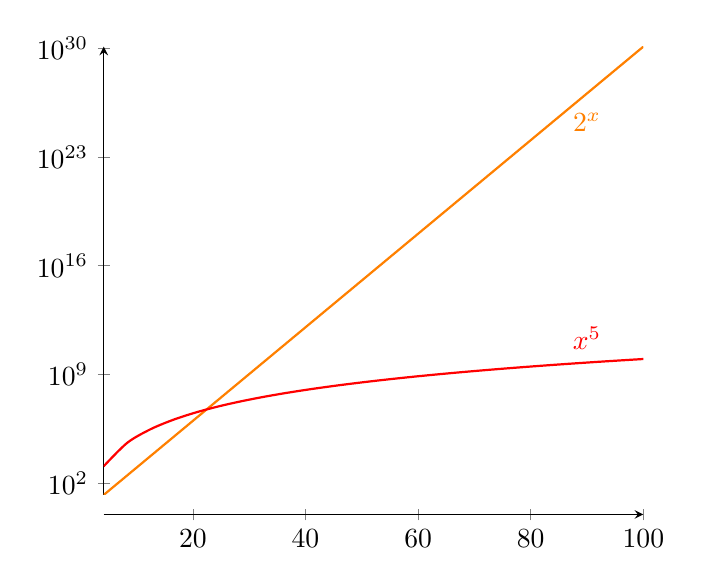
\begin{tikzpicture}
	    			\begin{semilogyaxis}[axis lines=middle,restrict expr to domain={y}{10:1e50},unbounded coords=discard]
	    			\addplot[domain=0:100,smooth,thick,orange]{2^x};
	    			\node [anchor=south,color=orange] at (axis cs:90,10^24){$2^x$};
	    			\addplot[domain=0:100,smooth,thick,red]{x^5};
	    			\node [anchor=south,color=red] at (axis cs:90,10^10){$x^5$};
	    			\end{semilogyaxis}
	    \end{tikzpicture}
	    \newline
	    Polynomial functions like $x^5$ will always increase slower than exponential functions like $2^x$ towards $\infty$, therefore: \[\lim_{x\to\infty}\frac{x^5}{2^x}=0\]
	\end{center}
\end{document}